\section{LVish, informally}\label{s:quasi-informal}

\ifdefined\DISSERTATION
While LVars offer a deterministic programming model that allows
communication through a wide variety of data structures, they are not
powerful enough to express common algorithmic patterns, like fixpoint
computations, that require both positive and negative queries.
\fi
In
this section, \either{I}{we} explain our extensions to the LVars model at a high
level; Section~\ref{s:quasi-formal} then formalizes them.

\subsection{Asynchrony through event handlers}

Our first extension to LVars is the ability to do asynchronous,
event-driven programming through event handlers.  An \emph{event} for
an LVar can be represented by a lattice element; the event
\emph{occurs} when the LVar's current value reaches a point at or
above that lattice element.  An \emph{event handler} ties together an
LVar with a callback function that is asynchronously invoked whenever
some events of interest occur.

To illustrate how event handlers work, consider again the lattice of
Figure~\ref{f:lvars-example-lattices}(a) from \either{Chapter}{Section}~\ref{ch:lvars}.
Suppose that $\mathit{lv}$ is an LVar whose states correspond to this
lattice.  The expression

\vspace{-8mm}
\singlespacing
\begin{equation}
  \ADDHANDLER~\mathit{lv}~\{ 1, 3, 5, \dots \}~(\lam{x}{\putexp{\mathit{lv}}{x+1}})
\label{e:lvish-example-1}
\end{equation}
\doublespacing

\noindent registers a handler for $\mathit{lv}$ that executes the callback
function $\lam{x}{\putexp{\mathit{lv}}{x+1}}$ for each odd number that
$\mathit{lv}$ is at or above.  When \eref{e:lvish-example-1} is
finished evaluating, $\mathit{lv}$ will contain the smallest even
number that is at or above what its original value was.  For instance,
if $\mathit{lv}$ originally contains $4$, the callback function will
be invoked twice, once with $1$ as its argument and once with $3$.
These calls will respectively write $1+1 = 2$ and $3+1 = 4$ into
$\mathit{lv}$; since both writes are $\leq 4$, $\mathit{lv}$ will
remain $4$.  On the other hand, if $\mathit{lv}$ originally contains
$5$, then the callback will run three times, with $1$, $3$, and $5$ as
its respective arguments, and with the latter of these calls writing
$5+1 = 6$ into $\mathit{lv}$, leaving $\mathit{lv}$ as $6$.

In general, the second argument to @addHandler@, which \either{I}{we} call an
\emph{event set}, is an arbitrary subset $Q$ of the LVar's lattice,
specifying which events should be handled.\footnote{Like threshold
  sets, these event sets are a mathematical modeling tool only; they
  have no explicit existence in the LVish library implementation.}
Event handlers in the LVish model are somewhat unusual in that they
invoke their callback for \emph{all} events in their event set $Q$
that have taken place (\ie, all values in $Q$ less than or equal to
the current LVar value), even if those events occurred prior to the
handler being registered.  To see why this semantics is necessary,
consider the following, more subtle example (written in a hypothetical
language with a semantics similar to that of $\lambdaLVar$, but with
the addition of @addHandler@):

\vspace{-8mm}
\singlespacing
\begin{equation}
\begin{split}
& \LETPAR ~\_ = \putexp{\mathit{lv}}{0} \\
&  \letparspace ~\_ = \putexp{\mathit{lv}}{1} \\
&  \letparspace ~\_ = \ADDHANDLER~\mathit{lv}~\{ 0, 1 \}~
     (\lam{x}{\termfont{if}~x=0~\termfont{then}~\putexp{\mathit{lv}}{2}}) \\
&  \letspace \IN~ \getexp{\mathit{lv}}{\setof{2}}
\end{split}
\label{e:lvish-example-2}
\end{equation}
\doublespacing

Can~\eref{e:lvish-example-2} ever block?  If a callback only executed
for events that arrived after its handler was registered, or only for
the largest event in its event set that had occurred, then the
example would be nondeterministic: it would block, or not, depending
on how the handler registration was interleaved with the
\termfont{put}s.  By instead executing a handler's callback once for
\emph{each and every} element in its event set below or at the LVar's
value, we guarantee quasi-determinism---and, for
\eref{e:lvish-example-2}, guarantee the result of $2$.

The power of event handlers is most evident for lattices that model
collections, such as sets.  For example, if we are working with
lattices of sets of natural numbers, ordered by subset inclusion, then
we can write the following function:
\[
\termfont{forEach} = \lam{\mathit{lv}}{
  \lam{f}{
    \ADDHANDLER~\mathit{lv}~\{ \{0\}, \{1\}, \{2\}, \dots \}~f
  }}
\]
Unlike the usual @forEach@ function found in functional programming
languages, this function sets up a \emph{permanent}, asynchronous flow
of data from $\mathit{lv}$ into the callback $f$.  Functions like
@forEach@ can be used to set up complex, cyclic data-flow networks, as
we will see in \either{Chapter}{Section}~\ref{ch:lvish}.

In writing @forEach@, we consider only the singleton sets to be events
of interest, which means that if the value of $\mathit{lv}$ is some
set like $\setof{2, 3, 5}$ then $f$ will be executed once for each
singleton subset ($\setof{2}$, $\setof{3}$, $\setof{5}$)---that is,
once for each element.  In \either{Chapter}{Section}~\ref{ch:lvish}, we will see that
this kind of event set can be specified in a lattice-generic way, and
that it corresponds closely to our implementation strategy.

\subsection{Quiescence through handler pools}\label{subsection:quasi-quiescence}

Because event handlers are asynchronous, we need a separate mechanism
to determine when they have reached a \emph{quiescent} state, \ie,
when all callbacks for the events that have occurred have finished
running. Detecting
quiescence is crucial for implementing fixpoint computations.  To
build flexible data-flow networks, it is also helpful to be able to
detect quiescence of multiple handlers simultaneously.  Thus, our
design includes \emph{handler pools}, which are groups of event
handlers whose collective quiescence can be tested.

The simplest way to program with handler pools is to use a pattern
like the following:

\vspace{-8mm}
\singlespacing
\[
\begin{array}[t]{l}
\termfont{let}~\mathit{h}~=~\NEWPOOL \\
\letspace \termfont{in}
  \begin{array}[t]{l}
    \ADDHANDLERINPOOL~h~\mathit{lv}~Q~f; \\
    \QUIESCE~h
  \end{array}
\end{array}
\]
\doublespacing

\noindent where $\mathit{lv}$ is an LVar, $Q$ is an event set, and $f$ is a
callback.  Handler pools are created with the @newPool@ function, and
handlers are registered with @addHandlerInPool@, a variant of
@addHandler@ that takes a
\ifdefined\DISSERTATION
\begin{wrapfigure}{l}{1.8in}
\vspace{-1.5em}
\begin{center}
  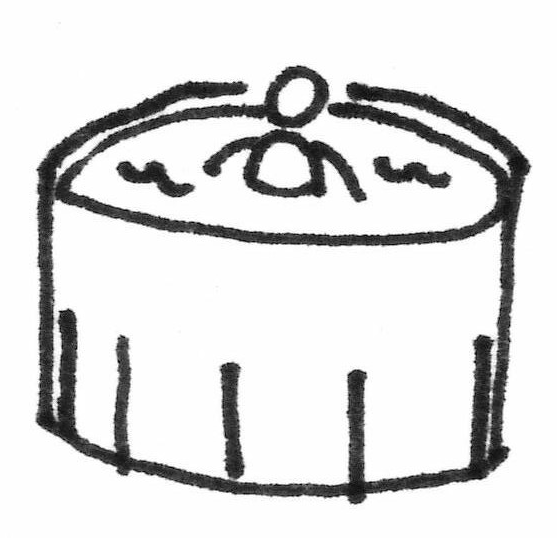
\includegraphics[scale=0.15]{../illustrations/pool}
\end{center}
\vspace{-2em}
\end{wrapfigure}
\fi
handler pool as an additional argument.
Finally, @quiesce@ takes a handler pool as its argument and blocks
until all of the handlers in the pool have reached a quiescent state.

Whether or not a handler is quiescent is a non-monotonic
property: we can move in and out of quiescence as more writes to an
LVar occur, and even if all states at or below the current state have
been handled, there is no way to know that more writes will not arrive
to move the LVar's state upwards in the lattice and trigger more
callbacks.  Early quiescence poses no risk to quasi-determinism, however,
because @quiesce@ does not yield any information about \emph{which}
events have been handled---any such questions must be asked through
LVar functions like @get@.  In practice, @quiesce@ is almost always
used together with freezing, which \either{I}{we} explain next.

\subsection{Freezing and the ``freeze-after'' pattern}\label{subsection:quasi-freeze-after}

Our final addition to the LVar model is the ability to \emph{freeze}
an LVar, which forbids further changes to it, but in return allows its
exact value to be read.  We expose freezing through the function
@freeze@, which takes an LVar as its sole argument and returns the
exact value of the LVar as its result.  Any writes that would change
the value of a frozen LVar instead raise an exception, and it is the
potential for races between such writes and @freeze@ that makes the
LVish model quasi-deterministic, rather than fully deterministic.

Putting all the above pieces together, we arrive at a particularly
common pattern of programming in the LVish model:

\vspace{-8mm}
\singlespacing
\[
\begin{array}[t]{l}
  \termfont{freezeAfter} = \lam{\mathit{lv}}{\lam{Q}{\lam{f}{}}}
  \begin{array}[t]{l}
    \termfont{let}~\mathit{h}~=~\NEWPOOL \\
    \letspace \termfont{in}
      \begin{array}[t]{l}  
        \ADDHANDLERINPOOL~h~\mathit{lv}~Q~f;
\\
        \QUIESCE~h;
\\
        \FREEZE~\mathit{lv}
      \end{array}
  \end{array}
\end{array}
\]
\doublespacing

\noindent In this pattern, an event handler is registered for an LVar,
subsequently quiesced, and then the LVar is frozen and its exact value
is returned.

\subsection{A parallel graph traversal using handlers, quiescence, and freezing}\label{subsection:quasi-parallel-graph-traversal}

We can use the new features in LVish to write a parallel graph
traversal in the simple fashion shown in
Listing~\ref{listing-bfs_new}.  This code, written using the LVish
Haskell library, discovers (in parallel) the set of nodes in a graph
@g@ reachable from a given node @startNode@, and is guaranteed to
produce a deterministic result.  It works by first creating a new
LVar, @seen@, to represent the set of seen nodes, then adding
@startNode@ to the set.  @newHandler@ is a helper function similar to
@addHandlerInPool@.  It takes the LVar @seen@ as its first argument,
and its second argument is the callback to be run whenever an event
occurs (that is, whenever a new element is added to the set of seen
nodes): for each new element that is seen, we look up its neighbors in
@g@ and then insert each of those elements into the set of seen nodes
as well.  The computation continues until there are no more events to
handle and @quiesce h@ returns.  We will return to this example in
Section~\ref{s:lvish-api}, which discusses the LVish library API in
more detail.

\singlespacing
\lstinputlisting[float, caption={A deterministic parallel graph traversal that uses \il{runParThenFreeze}.}, label=listing-bfs_new]{chapter3/code/bfs_new.hs}
\doublespacing
